\documentclass[tikz,border=0pt]{standalone}
% Shared look for the README diagrams. Colours are the app's own tokens (web/styles.css).
\usepackage[T1]{fontenc}
\usepackage[scaled=0.95]{helvet}
\renewcommand{\familydefault}{\sfdefault}
\usepackage{amsmath,amssymb}
\usepackage{tikz}
\usetikzlibrary{arrows.meta,positioning,fit,backgrounds,calc,shapes.geometric,shapes.symbols}

\definecolor{ink}{HTML}{15233F}
\definecolor{inksoft}{HTML}{3A4D6B}
\definecolor{paper}{HTML}{D9E7EF}
\definecolor{paperdeep}{HTML}{C6DAE6}
\definecolor{rule}{HTML}{9DB8CB}
\definecolor{safe}{HTML}{17643A}
\definecolor{safewash}{HTML}{D3EBDC}
\definecolor{caution}{HTML}{7A4F00}
\definecolor{cautionwash}{HTML}{F3DFA6}
\definecolor{danger}{HTML}{B0221B}
\definecolor{dangerwash}{HTML}{F7DCD9}
\definecolor{stop}{HTML}{8D0C0C}
\definecolor{stopwash}{HTML}{F6D4CF}
\definecolor{coral}{HTML}{FF8A80}
\definecolor{canvas}{HTML}{F7FAFC}

\newcommand{\modtitle}[1]{{\small\bfseries #1}}
\newcommand{\grouptag}[1]{{\scriptsize\bfseries\color{inksoft}\MakeUppercase{#1}}}

\tikzset{
  every node/.style={font=\footnotesize, text=ink},
  mod/.style={draw=ink, line width=0.7pt, fill=white, rounded corners=3pt, align=center,
              minimum height=1.25cm, inner sep=4pt},
  api/.style={mod, fill=paper},
  actor/.style={mod, fill=ink, text=white, minimum width=2.8cm},
  frame/.style={draw=rule, line width=0.8pt, dashed, rounded corners=6pt, inner sep=10pt},
  flow/.style={-{Stealth[length=6pt,width=5pt]}, line width=0.8pt, draw=ink},
  soft/.style={flow, draw=inksoft, dashed},
  halo/.style={preaction={draw=canvas, line width=4pt, -}},
  lab/.style={font=\scriptsize, text=inksoft, fill=canvas, inner sep=1.5pt},
  store/.style={cylinder, shape border rotate=90, aspect=0.18, draw=ink, line width=0.7pt,
                fill=paper, align=center, minimum height=1.35cm, inner sep=4pt},
}

% Light card behind everything (own layer, under the frames), so the SVG reads on GitHub's dark theme too.
\pgfdeclarelayer{card}
\pgfsetlayers{card,background,main}
\newcommand{\card}{%
  \begin{pgfonlayer}{card}
    \fill[canvas, rounded corners=10pt]
      ($(current bounding box.south west)+(-0.5,-0.5)$) rectangle ($(current bounding box.north east)+(0.5,0.5)$);
  \end{pgfonlayer}}
% code names without a bitmap typewriter font
\newcommand{\code}[1]{{\color{inksoft}\itshape #1}}
\begin{document}
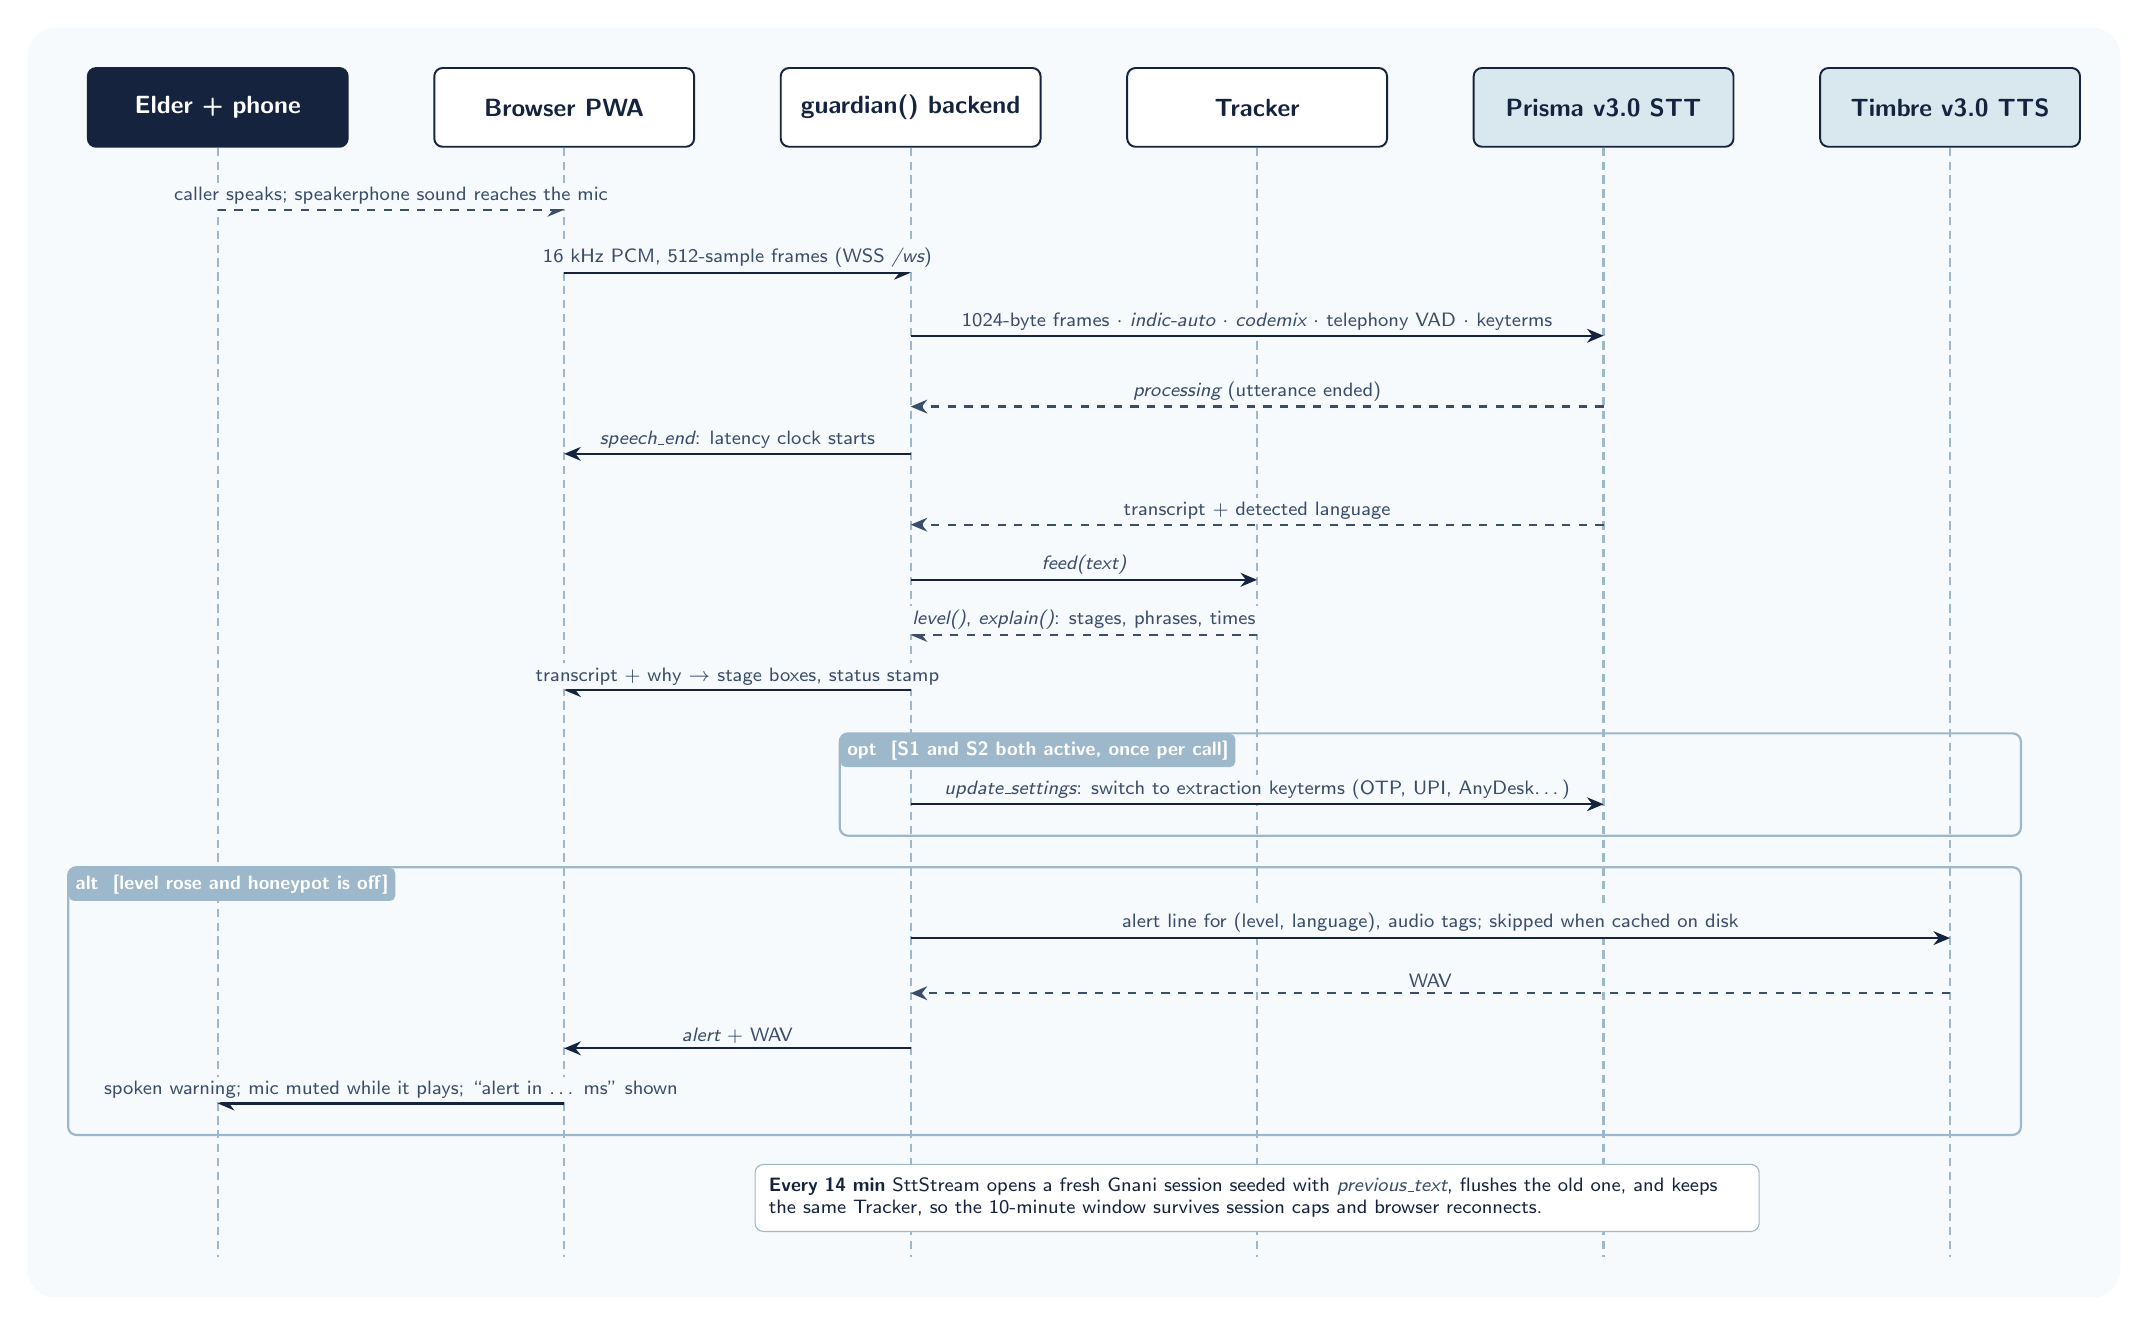
\begin{tikzpicture}[x=1cm,y=1cm,
  head/.style={minimum width=3.3cm, minimum height=1.0cm},
  msg/.style={flow},
  ret/.style={flow, dashed, draw=inksoft},
  m/.style={lab, above=0pt},
  box/.style={draw=rule, line width=0.8pt, rounded corners=3pt},
  boxlab/.style={fill=rule, text=white, font=\scriptsize\bfseries, inner sep=2.5pt, rounded corners=2pt, anchor=north west}]

\def\bot{-14.6}
\foreach \x/\n/\t/\s in {0/ph/Elder + phone/actor, 4.4/br/Browser PWA/mod, 8.8/be/guardian() backend/mod, 13.2/tr/Tracker/mod, 17.6/pr/Prisma v3.0 STT/api, 22.0/tb/Timbre v3.0 TTS/api} {
  \node[\s, head] (\n) at (\x,0) {\modtitle{\t}};
  \draw[rule, line width=0.8pt, dash pattern=on 3pt off 2pt] (\n.south) -- (\x,\bot);
}

% ---- streaming ------------------------------------------------------------------
\draw[ret] (0,-1.3) -- node[m] {caller speaks; speakerphone sound reaches the mic} (4.4,-1.3);
\draw[msg] (4.4,-2.1) -- node[m] {16 kHz PCM, 512-sample frames (WSS \code{/ws})} (8.8,-2.1);
\draw[msg] (8.8,-2.9) -- node[m] {1024-byte frames $\cdot$ \code{indic-auto} $\cdot$ \code{codemix} $\cdot$ telephony VAD $\cdot$ keyterms} (17.6,-2.9);
\draw[ret] (17.6,-3.8) -- node[m] {\code{processing} (utterance ended)} (8.8,-3.8);
\draw[msg] (8.8,-4.4) -- node[m] {\code{speech\_end}: latency clock starts} (4.4,-4.4);
\draw[ret] (17.6,-5.3) -- node[m] {transcript + detected language} (8.8,-5.3);
\draw[msg] (8.8,-6.0) -- node[m] {\code{feed(text)}} (13.2,-6.0);
\draw[ret] (13.2,-6.7) -- node[m] {\code{level()}, \code{explain()}: stages, phrases, times} (8.8,-6.7);
\draw[msg] (8.8,-7.4) -- node[m] {transcript + why $\rightarrow$ stage boxes, status stamp} (4.4,-7.4);

% ---- stage-following keyterms ------------------------------------------------------
\draw[box] (7.9,-7.95) rectangle (22.9,-9.25);
\node[boxlab] at (7.9,-7.95) {opt \ [S1 and S2 both active, once per call]};
\draw[msg] (8.8,-8.85) -- node[m] {\code{update\_settings}: switch to extraction keyterms (OTP, UPI, AnyDesk\ldots)} (17.6,-8.85);

% ---- alert ---------------------------------------------------------------------------
\draw[box] (-1.9,-9.65) rectangle (22.9,-13.05);
\node[boxlab] at (-1.9,-9.65) {alt \ [level rose and honeypot is off]};
\draw[msg] (8.8,-10.55) -- node[m] {alert line for (level, language), audio tags; skipped when cached on disk} (22.0,-10.55);
\draw[ret] (22.0,-11.25) -- node[m] {WAV} (8.8,-11.25);
\draw[msg] (8.8,-11.95) -- node[m] {\code{alert} + WAV} (4.4,-11.95);
\draw[msg] (4.4,-12.65) -- node[m] {spoken warning; mic muted while it plays; ``alert in \ldots\ ms'' shown} (0,-12.65);

% ---- rotation note -------------------------------------------------------------------
\node[draw=rule, fill=white, rounded corners=3pt, align=left, font=\scriptsize, text width=12.4cm, inner sep=5pt]
  at (13.2,-13.85) {\textbf{Every 14 min} SttStream opens a fresh Gnani session seeded with \code{previous\_text}, flushes the old one,
  and keeps the same Tracker, so the 10-minute window survives session caps and browser reconnects.};

\card
\end{tikzpicture}
\end{document}
